\begin{activity}{Layered and Anisotropic Conductivity}

\section*{Purpose}
To see how anisotropy of thermal conductivity arises from simple geometric models of layered materials and how this is expressed in natural samples.

\section*{Learning Outcomes}

By the end of this activity, you should be able to:
\begin{itemize}
  \item Derive the effective conductivity of layered media when heat flows parallel or perpendicular to layering.
  \item Use real directional conductivity data to estimate an anisotropy factor and propose a functional form for how conductivity varies with angle.
\end{itemize}

\section*{Geological Context}
Layering can happen in many geological contexts and at all scales from sheets of mica to layers in a sedimentary basin.   This activity builds the theoretical bounds on that directional dependence, then checks them against real measurements.

\section*{Tasks}
\begin{questions}

  \question{Perpendicular Case: Heat Flow Across the Layering}

  Consider $N$ layers stacked with heat flowing perpendicular to the layering -- crossing every layer in turn, exactly as in Activity 8.A, but now for an arbitrary number of layers rather than two. Layer $i$ has thickness $h_i$ and conductivity $k_i$; the interface temperatures are $T_0$ (top) through $T_N$ (base), and $H=\sum_i h_i$.

  \begin{center}
  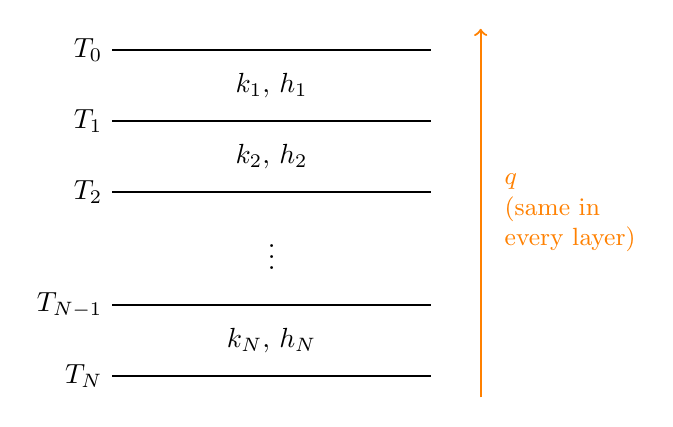
\begin{tikzpicture}[scale=0.9]
    \def\w{4.5}
    \draw[thick] (0,0) -- (\w,0);
    \draw[thick] (0,-1) -- (\w,-1);
    \draw[thick] (0,-2) -- (\w,-2);
    \draw[thick] (0,-3.6) -- (\w,-3.6);
    \draw[thick] (0,-4.6) -- (\w,-4.6);

    \node at (\w/2,-0.5) {$k_1,\,h_1$};
    \node at (\w/2,-1.5) {$k_2,\,h_2$};
    \node at (\w/2,-2.8) {$\vdots$};
    \node at (\w/2,-4.1) {$k_N,\,h_N$};

    \node[left] at (0,0) {$T_0$};
    \node[left] at (0,-1) {$T_1$};
    \node[left] at (0,-2) {$T_2$};
    \node[left] at (0,-3.6) {$T_{N-1}$};
    \node[left] at (0,-4.6) {$T_N$};

    \draw[->, orange, thick] (\w+0.7,-4.9) -- (\w+0.7,0.3);
    \node[orange, right, align=left, font=\small] at (\w+0.9,-2.3) {$q$\\(same in\\every layer)};
  \end{tikzpicture}
  \end{center}

  \begin{enumerate}[label=(\alph*)]
    \item In steady state with no internal heat production, what must be true about $q$ at every interface between layers, and why?
    \answerbox[1.5cm]

    \item Heat flows upward, from $T_N$ at the base toward $T_0$ at the top, so $T_N > T_0$: temperature increases with depth. Write Fourier's law for the temperature drop $\Delta T_i = T_i - T_{i-1}$ across layer $i$ alone (positive, since the deeper interface is hotter), in terms of $q$, $k_i$, and $h_i$.
    \answerbox[1.5cm]

    \item The total drop across the whole stack, in the direction heat is flowing, is $\Delta T = T_N - T_0$. How does $\Delta T$ relate to the individual $\Delta T_i$?
    \answerbox[1.5cm]

    \item Combine (b) and (c) to write $\Delta T$ as a single sum over all $N$ layers.
    \answerbox[2cm]

    \item Define an effective conductivity $k_\perp$ by requiring the whole stack obey Fourier's law as if it were one layer: $\Delta T = qH/k_\perp$. Set this equal to your result from (d) and solve for $1/k_\perp$.
    \answerbox[2.5cm]
  \end{enumerate}

  You should arrive at
  \begin{equation}
    \frac{1}{k_\perp} = \sum_{i=1}^N \frac{f_i}{k_i}, \qquad f_i \equiv \frac{h_i}{H}.
  \end{equation}
  This is the thickness-weighted \emph{harmonic mean} -- the same result as for two layers, but it fell out of the derivation for arbitrary $N$ with no extra work, since the sum in (d) was already general.

  \question{Parallel Case: Heat Flow Along the Layering}

  Now consider the \emph{same} stack of layers, but with heat flowing along the layering instead -- parallel to strike, not across it. Each layer independently carries its own share of the heat flow between two shared end temperatures $T_A$ and $T_B$.

  \begin{center}
  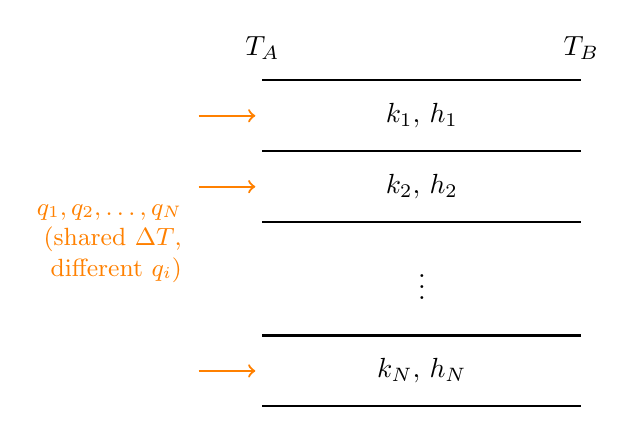
\begin{tikzpicture}[scale=0.9]
    \def\w{4.5}
    \draw[thick] (0,0) -- (\w,0);
    \draw[thick] (0,-1) -- (\w,-1);
    \draw[thick] (0,-2) -- (\w,-2);
    \draw[thick] (0,-3.6) -- (\w,-3.6);
    \draw[thick] (0,-4.6) -- (\w,-4.6);

    \node at (\w/2,-0.5) {$k_1,\,h_1$};
    \node at (\w/2,-1.5) {$k_2,\,h_2$};
    \node at (\w/2,-2.8) {$\vdots$};
    \node at (\w/2,-4.1) {$k_N,\,h_N$};

    \node[above] at (0,0.15) {$T_A$};
    \node[above] at (\w,0.15) {$T_B$};

    \draw[->, orange, thick] (-0.9,-0.5) -- (-0.1,-0.5);
    \draw[->, orange, thick] (-0.9,-1.5) -- (-0.1,-1.5);
    \draw[->, orange, thick] (-0.9,-4.1) -- (-0.1,-4.1);
    \node[orange, left, align=right, font=\small] at (-1.0,-2.3) {$q_1,q_2,\ldots,q_N$\\(shared $\Delta T$,\\different $q_i$)};
  \end{tikzpicture}
  \end{center}

  \begin{enumerate}[label=(\alph*)]
    \item What quantity is now shared by every layer -- not $q$ this time, but something else? (Compare to part (a) of Question 1: there, $q$ was forced to be equal across every layer. What plays that role here?)
    \answerbox[1.5cm]

    \item Heat flows from $T_A$ toward $T_B$, so $T_A > T_B$. Write Fourier's law for the heat flow $q_i$ carried by layer $i$, in terms of the shared gradient $g = (T_A-T_B)/\Delta x$ (positive, in the direction heat is flowing) and $k_i$.
    \answerbox[1.5cm]

    \item Each layer contributes $q_i h_i$ (its flux times its own thickness) to the total heat flow through the stack's cross-section. Write $Q_\text{total}$ as a sum over all $N$ layers.
    \answerbox[2cm]

    \item Define $k_\parallel$ by requiring the whole stack carry $Q_\text{total} = k_\parallel\, g\, H$. Solve for $k_\parallel$.
    \answerbox[2cm]
  \end{enumerate}

  You should arrive at
  \begin{equation}
    k_\parallel = \sum_{i=1}^N f_i k_i,
  \end{equation}
  the thickness-weighted \emph{arithmetic mean} -- and notice this one required no manipulation of reciprocals at all; the sum was already in the right form from step (c).

  \question{Numeric Check}

  A layered sequence has the properties below.

  \begin{center}
  \begin{tabular}{ccccc}
  \toprule
  Layer & 1 & 2 & 3 & 4 \\
  \midrule
  $h_i$ (m) & 12 & 4 & 20 & 8 \\
  $k_i$ (W\,m$^{-1}$K$^{-1}$) & 1.2 & 7.0 & 1.5 & 5.0 \\
  \bottomrule
  \end{tabular}
  \end{center}

  \begin{enumerate}[label=(\alph*)]
    \item Compute $k_\perp$ (perpendicular, across-layering) for this sequence.
    \answerbox[3cm]

    \item Compute $k_\parallel$ (parallel, along-layering) for the same sequence.
    \answerbox[3cm]

    \item Which is larger? By roughly what factor?
    \answerbox[1.5cm]

    \item This ordering, $k_\parallel \ge k_\perp$, holds for \emph{any} set of positive $k_i$ -- it's the arithmetic-mean/harmonic-mean inequality, a general mathematical fact, not a coincidence of these numbers. Physically, why should heat flowing \emph{along} the layering always manage a higher effective conductivity than heat forced \emph{across} it? (Hint: think about how much choice the heat has in each case about which layers carry it.)
    \answerbox[2.5cm]
  \end{enumerate}

  \question{Real Data: Directional Conductivity in Foliated Rocks}

  Many metamorphic rocks develop a strong planar fabric---foliation---during deformation, aligning platy minerals (especially micas) into a preferred orientation.

  The figure below shows measured thermal conductivity versus the angle between the measurement direction and foliation, for four samples: three metapelites and one gneiss.

  \begin{figure}[h]
      \centering
      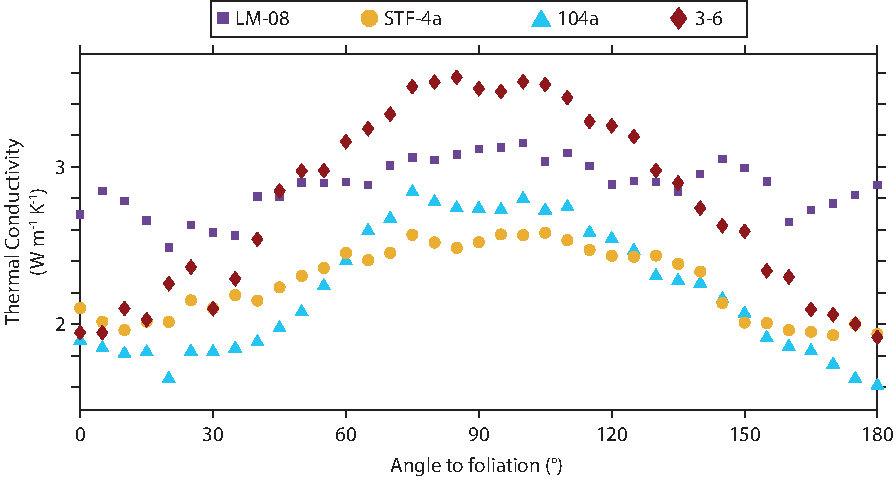
\includegraphics[width=0.8\textwidth]{figures/observed_anisotropy_angle.pdf}
      \caption{Thermal conductivity vs.\ angle to foliation for three metapelites and one gneiss.}
      \label{fig:aniso}
  \end{figure}

  \begin{enumerate}[label=(\alph*)]
    \item At $0^\circ$, is the measurement direction along the foliation plane or across it? What about $90^\circ$? State your reasoning -- don't just guess the convention.
    \answerbox[2.5cm]

    \item Using your answer to (a) together with Questions 1 and 2, which angle should correspond to $k_\parallel$ and which to $k_\perp$?
    \answerbox[2cm]

    \item Does the real data fall between the bounds you'd expect, or does something surprise you? Where do the curves peak?
    \answerbox[2.5cm]

    \item Define the \textbf{anisotropy factor} as $A = k_\text{max}/k_\text{min}$ for a given sample. Estimate $A$ for each of the four samples by reading approximate maximum and minimum conductivities off the figure.
    \answerbox[3cm]

    \item Compare $A$ across the three metapelites and the one gneiss. Is one rock type consistently more anisotropic than the other? Suggest a reason, connected to how each rock's fabric actually formed.
    \answerbox[2.5cm]

    \item Propose a simple mathematical function $k(\theta)$ that (i) equals your two derived bounds at the two extreme angles, and (ii) varies smoothly in between. You don't need to fit it precisely -- just propose a reasonable functional form and justify why you chose it.
    \answerbox[3cm]
  \end{enumerate}

\end{questions}

\section*{Key Ideas}

\textbf{The same physical setup gives different effective properties depending on flow direction.} Heat flowing across layering shares the same flux and sums temperature drops (harmonic mean); heat flowing along layering shares the same gradient and sums fluxes (arithmetic mean). Recognizing \emph{which quantity is common} to every layer is the whole derivation -- the mean falls out mechanically once that's identified.

\textbf{Parallel flow can always exploit the fastest pathway; perpendicular flow cannot avoid the slowest one.} $k_\parallel \ge k_\perp$ always, because along-layering heat is free to concentrate disproportionately in the highest-conductivity layers, while across-layering heat has no choice but to cross every layer, including the most resistive one, at the same rate as all the others.

\textbf{Real anisotropic media are not obligated to sit inside an idealized two-direction bound.} The harmonic/arithmetic bracket comes from treating a rock as alternating layers of two conductivities. Real foliated rocks carry additional anisotropy from the crystal-scale conductivity of their constituent minerals, so the true directional dependence is a combination of layering geometry and mineral fabric, not layering geometry alone.

\end{activity}
